%-----------------------------------------------
% Dateiname: Protype.tex
% Autor    : Stefano Kowalke <blueduck@gmx.net>
% Lizenz   : BSD
%-----------------------------------------------
\chapter{Prototypischer Nachweis der Herstellbarkeit}
\label{ch:protoype}

\begin{figure}[H]
    \centering
    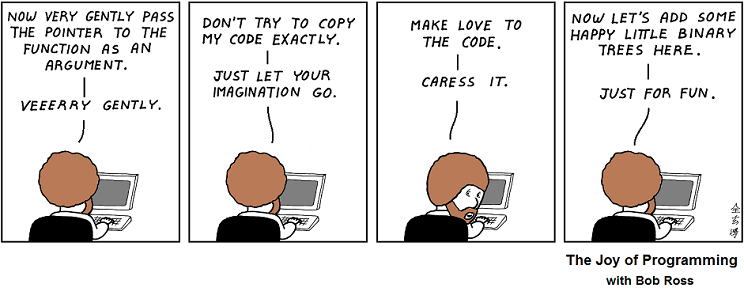
\includegraphics[scale=0.65]{gfx/the_art_of_happy_programming.png}
    \label{fig:bobRoss}
\end{figure}

Die Erstellung des Prototyps begann mit der Definition verschiedener Zielstellungen. Diese wurden in zusammenhängenden Arbeitspaketen zusammengefasst und dienten als Meileinsteine.

%-----------------------------------------------
% Dateiname: Concept.tex
% Autor    : Stefano Kowalke <blueduck@gmx.net>
% Lizenz   : BSD
%-----------------------------------------------
\section{Konzeption des Prototypen}
\label{prototype:sec:concept}
Bevor mit der Implementierung des Prototyps begonnen werden konnte, wurden die zu erreichenden Ziele definiert.

\begin{itemize}
\item Der Prototyp erhält den Extensionkey \textit{doctrine\_dbal}.
\item  Der Prototyp ist eine normale Extension, die über das \textit{Install Tool} installierbar ist. Dies ist notwendig, da bereits bei der Installation das zu nutzende \gls{dbms} auswählbar sein muß. Er ist gegenfalls ohne größeren Aufwand in eine Systemextension umwandelbar.
\item Der Prototyp unterstützt die alte Datenbank \gls{api}, damit TYPO3 CMS und externe Extensions weiterhin funktionieren.
\item Der Prototyp unterstützt MySQL als \gls{dbms}.
\item Die Methodennamen der neuen \gls{api} folgen den TYPO3 \gls{cgl}.
\item Die Erstellung der Basisdatenbank erfolgt durch Doctrine DBAL und nutzt dessen abstaktes Datenbankschema.
\item Der Prototyp nutzt intern \textit{Prepared Statements}.
\item Der Prototyp führt eine \textit{Fluent Query Language} ein, damit auf die manuelle Formulierung von SQL Anfragen verzichtet werden kann.
\end{itemize}

Diese Anforderungen konnten anschließend in einzelne Teilaufgaben zusammengefasst werden:

\begin{enumerate}
\item Erhöhung der Testabdeckung der vorhandenen Datenbank \gls{api}
\item Erstellen der Grundstrukutur des Prototypen
\item Integration in das \phpinline{Install Tool}
\item Implementation einer Fluent \gls{api}
\item Umbau von TYPO3 CMS auf die \gls{api} des Prototypen
\end{enumerate}


%\section{Refactoring der alten Datenbank API}
%\subsection{Tests für die alte Datenbank API}

%\section{Testgetriebene Implementierung der neuen Datenbank API}
%- Adapter
%- alte API Klasse erbt von neuer API Klasse
%- Verbindung mit der Datenbank via Doctrine
%- Methodenübername wenn sinnvoll
%- Neue Methoden

%\subsection{Einführung von Query Objekten}
%\subsubsection{SELECT}
%\subsubsection{INSERT}
%\subsubsection{UPDATE}
%\subsubsection{DELETE}
%\subsubsection{TRUNCATE}

%\section{Anwendung der neuen Datenbank API}
%\subsection{Anpassungen an TYPO3}
%\section{Überprüfen der Funktionalität}
%-----------------------------------------------
% Dateiname: InstallTYPO3.tex
% Autor    : Stefano Kowalke <blueduck@gmx.net>
% Lizenz   : BSD
%-----------------------------------------------
\section{Vorbereitung}
\label{prototype:sec:preparation}

\subsection{Installation von TYPO3 CMS}
\label{prototype:subsec:installTYPO3}
TYPO3 CMS wurde auf dem lokalen Rechner per \textit{GIT} in der Entwicklerversion 6.2.x-dev unter \url{thesis.dev} installiert. TYPO3 CMS 6.2 stellte die zum Zeitpunkt der Implementierung aktuelle Version dar. Die Entwicklerversion wurde gewählt, um von der fortlaufenden Weiterentwicklung des Systems zu profitieren. \textit{GIT} wurde verwendet, damit der Code einfacher aktualisierbar war und eigene Änderungen daran nachvollzogen und dokumentiert werden konnten.

Abbildung~\ref{lst:thesisDevFolders} zeigt die Verzeichnisstruktur nachdem das System installiert und alle notwendigen Verzeichnisse und Symlinks erstellt wurden:

\begin{figure}[H]
\begin{Verbatim}[samepage=true]
$ tree -L 2 --dirsfirst
.
├── http
│   ├── fileadmin
│   ├── typo3 -> typo3_src/typo3
│   ├── typo3_src -> ../typo3cms
│   ├── typo3conf
│   ├── uploads
│   └── index.php -> typo3_src/index.php
└── typo3cms
    ├── typo3
    ├── ChangeLog
    ├── GPL.txt
    ├── INSTALL.md
    ├── LICENSE.txt
    ├── NEWS.md
    ├── README.md
    ├── _.htaccess
    ├── composer.json
    └── index.php
\end{Verbatim}
\caption{Die Grundstruktur von \url{thesis.dev}}
\label{lst:thesisDevFolders}
\end{figure}

Das Verzeichnis \pdf{http} wurde per Eintrag in der Apache2 Konfiguration als VirtualHost definiert.

\begin{shcode}
<VirtualHost *:80>¬
DocumentRoot "~/Sites/thesis.dev/http"¬
ServerName thesis.dev¬
</VirtualHost>
\end{shcode}

TYPO3 CMS wurde nach \pdf{typo3cms} installiert, damit dessen Dateien nicht über den Apache ereichbar sind.

Um die Installation unter der Adresse \url{thesis.dev} erreichen zu können, wurde in der Hostdatei ein A-Record angelegt.

\begin{shcode}
sudo sh -c "echo '127.0.0.1 thesis.dev' >> /etc/hosts"
\end{shcode}

Im Anschluß daran wurde eine leere Datenbank mit dem Namen \texttt{thesis} erstellt:

\begin{shcode}
mysql -u root -p
MariaDB [(none)]> create database if not exists thesis;
Query OK, 1 row affected (0.01 sec)
MariaDB [(none)]> quit;
\end{shcode}

Durch das Aufrufen von \url{http://thesis.dev/} im Browser wird der Installationsprozess gestartet, der in fünf Schritten das System installiert.

\subsection{Schritt 1 - Systemcheck}
	Im ersten Schritt (Abb.:~\ref{fig:installTYPO3LegacyStepOne}) prüft das \textit{Install Tool} ob alle Verzeichnisse und Symlinks angelegt wurden und die entsprechenden Benutzerrechte besitzen. Intern werden hier Verzeichnisse wie \pdf{typo3temp} und Dateien wie \pdf{LocalConfiguration.php} angelegt.

\subsection{Schritt 2 - Eingabe der Datenbankdaten}
	Im zweiten Schritt (Abb.:~\ref{fig:installTYPO3LegacyStepTwo}) werden die Benutzerdaten für die Datenbank eingegeben. Es kann zwischen einer Port- oder Socket-basierten Verbindung ausgewählt werden.

	Wenn anstelle von MySQL ein alternatives \gls{dbms} genutzt werden soll, kann über die Schaltfläche am Ende des Formulars die Systemextension DBAL installiert werden.

\subsection{Schritt 3 - Auswahl der Datenbank}
	Nachdem die Verbindungsdaten eingegeben wurden, versucht TYPO3 CMS eine Verbinung zum \gls{dbms} zu etablieren. Gelingt dies, werden alle verfügbaren Datenbanken abgefragt und aufgelistet (Abb.:~\ref{fig:installTYPO3LegacyStepThree}). Über die Auswahl kann eine leere Datenbank festgelegt werden. Alternativ kann über das Inputfeld eine zu erstellende Datenbank angegeben werden. Mit dem Absenden des Formulars werden die Basistabellen in der Datenbank angelegt.

\subsection{Schritt 4 - Einrichten eines TYPO3 Administrators}
	In 4. Schritt (Abb.:~\ref{fig:installTYPO3LegacyStepFour}) der Installation wird ein Administrator eingerichtet und es kann ein Name für die Seite vergeben werden.

\subsection{Schritt 5 - Abschluß der Installation}
	Danach ist die Installation abgeschlossen und über die Schaltfläche kann das Backend aufgerufen werden (Abb.:~\ref{fig:installTYPO3LegacyStepFive})

	\begin{figure}[H]
		\begin{subfigure}[b]{0.5\textwidth}
			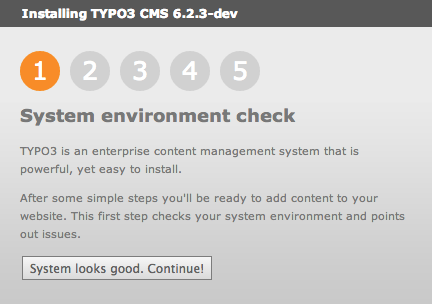
\includegraphics[width=\textwidth]{InstallingTYPO3/DoctrineDBAL/01-SystemEnvironmentCheck.png}
			\caption{Installation TYPO3 CMS - 1. Schritt}
			\label{fig:installTYPO3LegacyStepOne}
		\end{subfigure}%
		~ %add desired spacing between images, e. g. ~, \quad, \qquad, \hfill etc.
	%(or a blank line to force the subfigure onto a new line)
		\begin{subfigure}[b]{0.5\textwidth}
			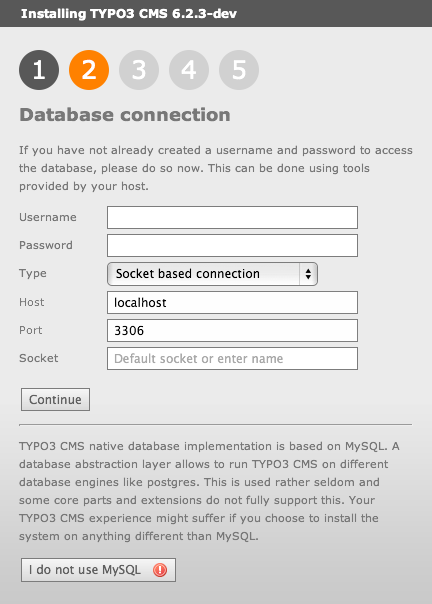
\includegraphics[width=\textwidth]{InstallingTYPO3/Legacy/02-DatabaseConnectionLegacy.png}
			\caption{Installation TYPO3 CMS - 2. Schritt}
			\label{fig:installTYPO3LegacyStepTwo}
		\end{subfigure}
		~ %add desired spacing between images, e. g. ~, \quad, \qquad, \hfill etc.
	%(or a blank line to force the subfigure onto a new line)
		\begin{subfigure}[b]{0.5\textwidth}
			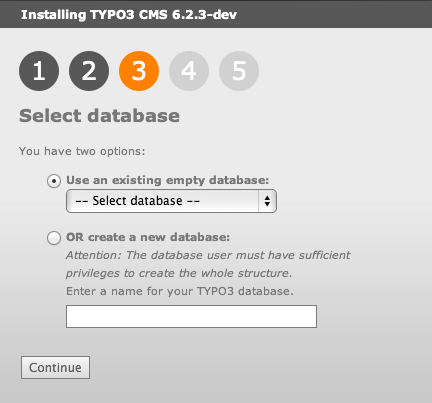
\includegraphics[width=\textwidth]{InstallingTYPO3/Legacy/03-SelectDatabaseLegacy.png}
			\caption{Installation TYPO3 CMS - 3. Schritt}
			\label{fig:installTYPO3LegacyStepThree}
		\end{subfigure}%
		~ %add desired spacing between images, e. g. ~, \quad, \qquad, \hfill etc.
	%(or a blank line to force the subfigure onto a new line)
		\begin{subfigure}[b]{0.5\textwidth}
			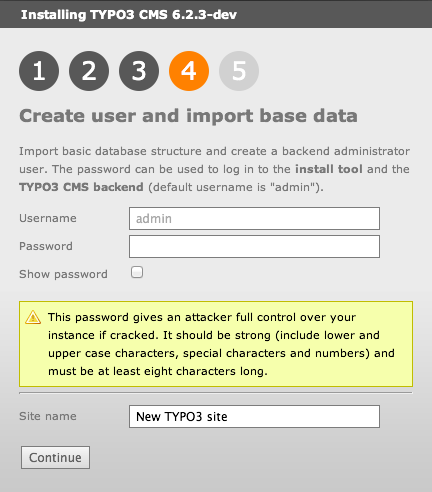
\includegraphics[width=\textwidth]{InstallingTYPO3/Legacy/04-CreateUserAndImportBaseDataLegacy.png}
			\caption{Installation TYPO3 CMS - 4. Schritt}
			\label{fig:installTYPO3LegacyStepFour}
		\end{subfigure}
		~ %add desired spacing between images, e. g. ~, \quad, \qquad, \hfill etc.
	%(or a blank line to force the subfigure onto a new line)
		\begin{subfigure}[b]{0.5\textwidth}
			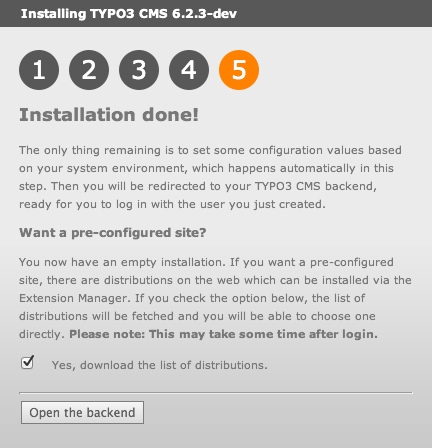
\includegraphics[width=\textwidth]{InstallingTYPO3/Legacy/05-InstallationDoneLegacy.png}
			\caption{Installation TYPO3 CMS - 5. Schritt}
			\label{fig:installTYPO3LegacyStepFive}
		\end{subfigure}%
		\caption{Installation von TYPO3 CMS}
		\label{fig:installationOfTYPO3}
	\end{figure}

\subsection{Implementation von Unit Tests der alten Datenbank API}
\label{prototype:sec:createTestForOldAPI}
Um zu gewährleisten, dass TYPO3 CMS sowohl mit der alten API - die von dem Prototypen zur Verfügung gesellt wird - als auch mit der neuen API kompatibel ist, müssen Untit Tests für die alte Datenbank API geschrieben werden.

Zur Ausführung der Unit Tests wird die Extension \textit{PHPUnit} benötigt, welche das gleichnamige Testing Framework \textit{PHPUnit\footnote{\url{http://www.phpunit.de}}} zur Verfügung und einen einen graphischen Testrunner im Backend mitbringt. Sie wird über den Extension Manager installiert.

Die alte Datenbank API verfügt zur dem Zeitpunkt der Erstelltung des Prototypen über 40 Tests mit 49 Assertions, welche jedoch lediglich Hilfsmethoden testen. Im Laufe der Arbeit wurden wurden 68 Tests implementiert, die alle Methoden testen. Die Abbildung~\ref{fig:executeUnitTestsForOldAPI} zeigt die Ausführung der von TYPO3 CMS mitgelieferten Unit Tests; Abbildung~\ref{fig:executeNewUnitTestsForOldAPI} zeigt die Ausführung der neu implementierten sowie der alten Tests.

\begin{figure}[H]
    \centering
    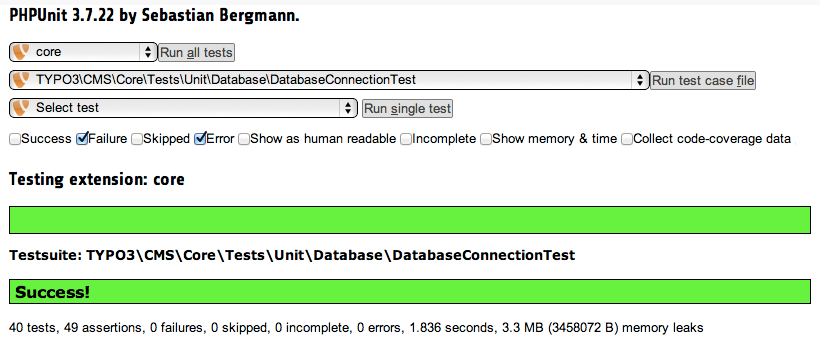
\includegraphics[scale=0.5]{TYPO3/DatabaseConnectionUnitTestsLegacy.png}
    \caption{Ausführung der vorhandenen Unit Tests für die alte Datenbank API}
    \label{fig:executeUnitTestsForOldAPI}
\end{figure}

\begin{figure}[H]
    \centering
    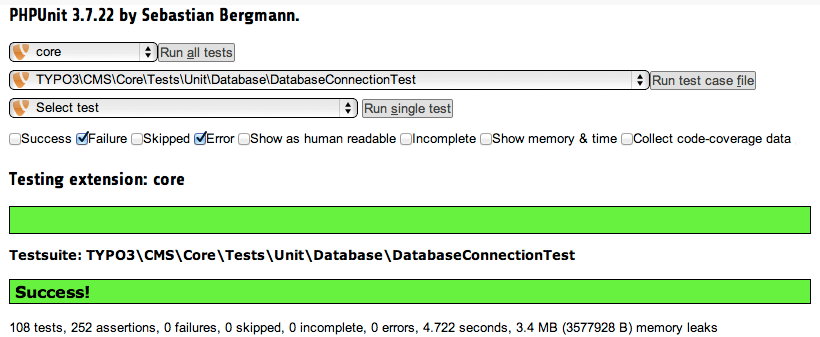
\includegraphics[scale=0.5]{TYPO3/DatabaseConnectionAddedUnitTestsLegacy.png}
    \caption{Ausführung der vorhandenen und hinzugefügten Unit Tests für die alte Datenbank API}
    \label{fig:executeNewUnitTestsForOldAPI}
\end{figure}

%-----------------------------------------------
% Dateiname: CreatePrototype.tex
% Autor    : Stefano Kowalke <blueduck@gmx.net>
% Lizenz   : BSD
%-----------------------------------------------
\section{Erstellung des Prototypen}
\label{prototype:sec:createPrototype}
Die Grundstruktur des Prototypen wurde unter \pdf{thesis/http/typo3conf/ext/doctrine\_dbal} erstellt.

\begin{Verbatim}[samepage=true]
.
└── doctrine_dbal/
    ├── Configuration/
    ├── Resources/
    ├── ext_emconf.php
    ├── ext_icon.gif
    └── ext_tables.php
\end{Verbatim}

Die Datei \pdf{ext\_emconf.php} enthält die Metainformationen der Extension, die vom Extension Manager verarbeitet werden.

\begin{listing}
\begin{phpcode}
<?php
$EM_CONF[$_EXTKEY] = array(
	'title' => 'Doctrine DBAL',
	'description' => 'Doctrine DBAL Integration in TYPO3 CMS',
	'category' => 'be',
	'author' => 'Stefano Kowalke',
	'author_email' => 'blueduck@gmx.net',
	'author_company' => 'Skyfillers GmbH',
	...
	'version' => '0.1.0',
	'constraints' => array(
		'depends' => array(
			'typo3' => '6.2.0-6.2.99',
		),
		'conflicts' => array('adodb', 'dbal'),
	...
	),
);
\end{phpcode}
\caption{Die Datei ext\_emconf.php}
\label{lst:extEmconf}
\end{listing}

Anschließend wurde Doctrine DBAL über \textit{Composer} installiert, indem es als externe Abhängigkeit in der \pdf{composer.json} definiert und durch das Kommando\\ \shinline{composer install} in den Ordner \pdf{vendor/doctrine} installiert wurde.

\begin{listing}[H]
\begin{jsoncode}
{
	"name": "typo3/doctrine_dbal",
	"type": "typo3-cms-extension",
	"description": "This brings Doctrine2 to TYPO3",
	"homepage": "http://typo3.org",
	"license": ["GPL-2.0+"],
	"version": "6.2.0",
	"require": {
		"doctrine/dbal": "dev-master"
	},
	"mininum-stability": "dev",
}
\end{jsoncode}
\caption{Die Datei composer.json}
\label{lst:composer}
\end{listing}


Die Integration von Doctrine DBAL sollte so transparent für TYPO3 CMS und die Extensions erfolgen, dass weiterhin über die Methoden der alten API auf die Datenbank zugegriffen werden kann. Die alte API steht dabei vergleichbar einer Fassade vor der neuen API, die ankommende Anfragen selbst behandelt oder an die neue API delegiert. Dieses Vorgehen erlaubt die sukzessive Integration von Doctrine DBAL.

Dazu wurde

\begin{itemize}
	\item im Ordner \pdf{doctrine\_dbal/Classes/Persistence/Doctrine} die Datei\\ \pdf{DatabaseConnection.php} erstellt (im weiteren Verlauf als \textit{neue API} bezeichnet),
	\item die Datei \pdf{DatabaseConnection.php} aus der Codebasis von TYPO3 CMS in den Ordner \pdf{doctrine\_dbal/Classes/Persistence/Legacy} des Prototypen kopiert (im weiteren Verlauf als \textit{alte API} bezeichnet),
	\item die Datei \pdf{DatabaseConnectionTests.php} aus der Codebasis von TYPO3 CMS in den Ordner \pdf{doctrine\_dbal/Tests/Persistence/Legacy} des Prototypen kopiert,
	\item eine Vererbung realisiert, die die Klasse der alten API von der Klasse der neuen API erben lässt (siehe Abb:.~\ref{fig:oldAPIextendsNewAPI} und
\begin{figure}[H]
    \centering
    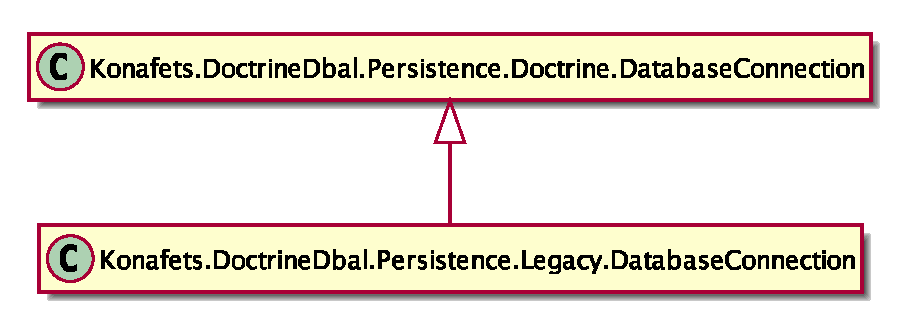
\includegraphics[scale=0.5]{gfx/uml/NewAPI/OldDatabaseConnectionExtentsFromNewAPI.eps}
    \caption{Alte API-Klasse erbt von neuer API-Klasse}
    \label{fig:oldAPIextendsNewAPI}
\end{figure}
	\item die Klasse der alten API per XCLASS in der Datei \pdf{ext\_localconf.php} registiert (Listing~\ref{lst:xclassDatabaseAPI}).
\end{itemize}


\begin{listing}[H]
\begin{phpcode}
if (!defined('TYPO3_MODE')) {
	die('Access denied.');
}

$GLOBALS['TYPO3_CONF_VARS']['SYS']['Objects']
  ['TYPO3\\CMS\\Core\\Database\\DatabaseConnection'] =
  array(
    'className' => 'Konafets\\DoctrineDbal\\Persistence\\Legacy\\DatabaseConnection');
\end{phpcode}
\caption{Registrierung der XCLASSes in \pdf{doctrine\_dbal/ext\_localconf.php}}
\label{lst:xclassDatabaseAPI}
\end{listing}

Danach wurden alle Eigenschaften aus der alten API in die neue API verschoben und mit Setter/Getter-Methoden versehen, die von der alten API ab diessem Zeitpunkt genutzt wurden.

Die Umstellung auf Doctrine begann mit dem Refactoring der Methode \phpinline{connectDB()} der alten API. Dabei wurde lediglich die Implementation der Methode vereinfacht, da sie unübersichtlich war und mehrere unterschiedliche Aufgaben ausführte, die nichts mit deren Aufgabengebiet - der Herstellung einer Verbindung zur Datenbank - gemein hatten.

Neben ihrer eigentlichen Aufgabe hast sie

\begin{itemize}
	\item einen Test durchgeführt, ob eine Datenbank konfiguriert ist
	\item die konfigurierte Datenbank ausgewählt und
	\item verschiedene Hooks ausgeführt
\end{itemize}

Code, der nicht zur definierten Aufgabe der Methode gehörte, wurde in eigene Methoden ausgelagert. Die Methode zur Überprüfung der veralteten Parameter konnte gänzlich entfallen, da die Änderungen an der neuen API stattfanden. Die Methode wurde anhand des aufgestellten Namensschemas umbenannt und wird von der alten Methode aufgerufen. Zusätzlich fängt die Methode nun die von Doctrine DBAL kommende Exception wenn keine Verbindung erstellt werden konnte und wirft eine eigene \phpinline{ConnectionException}. Die entsprechenden Exceptionklassen wurden in\\ \pdf{doctrine\_dbal/Classes/Exeptions/} erstellt. Listing~\ref{lst:connectDatabaseAfterRefactoring} zeigt die Methode nach dem Refactoring; Listing~\ref{lst:connectDBcallsConnectDatabase()} zeigt den Aufruf der neuen Methode.

\begin{listing}[H]
\begin{phpcode}
public function connectDatabase($isInitialInstallationInProgress = FALSE) {
	// Early return if connected already
	if ($this->isConnected) {
		return;
	}

	if (!$isInitialInstallationInProgress) {
		$this->checkDatabasePreconditions();
	}

	try {
		$this->link = $this->getConnection();
	} catch (\Exception $e) {
		throw new ConnectionException($e->getMessage());
	}

	$this->isConnected = $this->checkConnectivity();

	if (!$isInitialInstallationInProgress) {
		if ($this->isConnected) {
			$this->initCommandsAfterConnect();
			$this->selectDatabase();
		}

		$this->prepareHooks();
	}
}
\end{phpcode}
\caption{connectDatabase() nach dem Refactoring}
\label{lst:connectDatabaseAfterRefactoring}
\end{listing}

\begin{listing}[H]
\begin{phpcode}
public function connectDB(...) {
	...
	$this->connectDatabase();
}
\end{phpcode}
\caption{connectDB() delegiert an die neue API-Methode}
\label{lst:connectDBcallsConnectDatabase()}
\end{listing}

Die originale Implementation der Methode ist in \pdf{typo3/sysext/core/Classes/Database/DatabaseConnection.php} ab Zeile 1578 zu finden.\footnote{\url{http://bit.ly/typo3cms-legacy-connectdb}}

Die Erstellung der Verbindung wurde in der alten API an die Methode \phpinline{sql_pconnect()} ausgelagert. \phpinline{getConnection()} ist der Name der Methode die diese Aufgabe in der neuen API übernimmt.

Zunächst wurde Code, welcher nicht zum Aufgabengebiet der Methode gehört, in eigene Klassen ausgelagert. In dem Fall betraf das den Test nach einer installierten MySQLi PHP-Erweiterung, welcher im gleichen Zuge auf PDO geändert wurde. Die Initialisierung von Doctrine erfolgt in einer eigenen Methode. Dort wird je eine Instanz von \phpinline{\Doctrine\DBAL\Configuration} und \phpinline{\Doctrine\DBAL\Schema\Schema} erstellt. In der alten API bot Die Methode die Möglichkeit einer persistenten Verbindung zur Datenbank. Dies wurde implementiert, in dem ein eigenes \phpinline{PDO}-Objekt mit dem Konstrukturparameter \phpinline{\PDO::ATTR_PERSISTENT => true} erstellt und in dem Konfigurationsarray gespeichert wurde. Dieses Konfigurationsarray (siehe Listing~\ref{lst:DoctrineConfigArray}) wird\\ \phpinline{\Doctrine\DBAL\DriverManager::getConnection()} übergeben.

\begin{listing}[H]
\begin{phpcode}
protected $connectionParams = array(
	'dbname'   => '',
	'user'     => '',
	'password' => '',
	'host'     => 'localhost',
	'driver'   => 'pdo_mysql',
	'port'     => 3306,
	'charset'  => 'utf8',
);
\end{phpcode}
\caption{Das Konfigurationsarray für Doctrine DBAL}
\label{lst:DoctrineConfigArray}
\end{listing}

Zudem muß Doctrine DBAL der Datentyp \sqlinline{Enum} bekanntgemacht werden. Anschließend wird der Schema Manager erstellt, welcher zur Verwaltung des Datenbankschemas notwendig ist. Am Schluß wird das Verbindungsobjekt zurückgegeben.Der Code ist in \phpinline{\Konafets\DoctrineDbal\Persistence\Doctrine\DatabaseConnect::getConnection()}\footnote{\url{http://bit.ly/1sOXU1q}} zu finden.

Nachdem durch Doctrine DBAL die Verbindung hergestellt werden konnte, wurde die Methode \phpinline{query()} der alten API übernommen. Sie stellt die zentrale Schnittstelle aller API-Methoden zum Senden ihrer Anfragen an die Datenbank dar. Sie kapselt die gleichnamige Methode \phpinline{\Doctrine\DBAL\Connection::query()}.

\begin{listing}
\begin{phpcode}
protected function query($query) {
	if (!$this->isConnected) {
		$this->connectDatabase();
	}

	$stmt = $this->link->query($query);

	return $stmt;
}
\end{phpcode}
\caption{getConnection() der neuen API}
\label{lst:getConnectionNewAPI}
\end{listing}

Wie bereits in Kapitel~\ref{basics:doctrine:subsubsec:simpleDatabaseQueries} erwähnt wurde, gibt \phpinline{query()} ein Statementobjekt zurück, welches die Ergebnismenge bereithält. Dort wurde ebenfalls dargestellt, dass diese Menge durch die Methode \phpinline{fetch()} in Verbindung mit PDO-Konstanten in Index-basierte oder Assoziative Arrays formatiert werden kann.

Um die Arbeit mit der Ergebnismenge zu erleichtern wurden die drei Methoden\\ \phpinline{fetchAssoc($stmt)}, \phpinline{fetchRow($stmt)} und \phpinline{$fetchColumn($stmt)} implementiert, die die am Häufigsten vorkommenden  \textit{Fetch-Styles} kapseln.

\begin{phpcode}
public function fetchAssoc($stmt) {
	if ($this->debugCheckRecordset($stmt)) {
		return $stmt->fetch(\PDO::FETCH_ASSOC);
	} else {
		return FALSE;
	}
}
\end{phpcode}

Die ehemaligen \phpinline{admin_*}-Methoden wurden in \phpinline{list_*}-Methoden umbenannt, da die Unterscheidung in Admin und Nicht-Admin Methoden nicht nachvollziehbar war. Diese Mehoden stellen wichtige Metainformation zur darunterliegenden Datenbank bereit, die nicht nur für das \textit{Install Tool} von Nutzen sind.

Als Beipiel der Abstraktion, die Doctrine DBAL mitbringt, sei die Implementation der Methode \phpinline{listDatabases()} angeführt. Nach dem obligatorischen Verbindungstest, gibt der \phpinline{SchemaManager} eine Liste aller Datenbanken zurück - vollkommen unabhängig von der zugrundeliegenden \gls{dbms}.

\begin{phpcode}
public function listDatabases() {
	...
	$databases = $this->schemaManager->listDatabases();
    ...
	return $databases;
}
\end{phpcode}

Doctrine stellt zum Maskieren von Benutzereingaben die Methode\\ \phpinline{\Doctrine\DBAL\Connection::quote()} bereit. Im Gegensatz zur alten API, dessen Methode ein Backslash (\phpinline{\}) den zu maskierenden Zeichen voranstellt, werden die Zeichen von Doctrine durch ein Hochkomma (\phpinline{'}) maskiert. Die Methode \phpinline{\Doctrine\DBAL\Connection::quote()} wurde in der neuen API durch eine gleichnamige Methode gekapselt und stellt die Basis für alle weitere Methoden wie \phpinline{fullQuoteString()}, \phpinline{fullQuoteArray()}, \phpinline{quoteString()} und \phpinline{escapeStringForLike()} dar, welche das Verhalten der alten Methoden implementieren.

Die neue API bietet dagegen die Methoden \phpinline{quoteColumn()}, \phpinline{quoteTable()} und\\ \phpinline{quoteIdentifier()} zum Maskieren an. Es kann weiterhin\\ \phpinline{\Konafets\DoctrineDbal\Persistence\Doctrine\DatabaseConnection::quote()} genutzt werden; sicherer ist es jedoch von Anfang die Benutzung von Prepared Statements, welche von TYPO3 CMS seit Version 6.2 in Form eines Wrappers um die \textit{Prepared Statements} von MySQLi angeboten werden. Sie besitzen die gleichen API, wie sie in Kapitel~\ref{basics:doctrine:subsubsec:preparedStatements} vorgestellt wurde.

Durch den Aufruf der Methode \phpinline{$stmt = $GLOBALS['TYPO3_DB']->prepare($sql)} wird zunächst ein Objekt vom Typ \phpinline{\TYPO3\CMS\Core\Database\PreparedStatement} erstellt, dem der in \phpinline{$sql} gespeicherte Prepared Statemnt übergeben wird. Ein Aufruf von\\ \phpinline{$stmt->bind(':lastName', 'Potter')} fügt einem internen Array des Objekts diese Werte hinzu. Zusätzlich wird versucht den Datentyp zu erkennen und ebenfalls zu speichern. Erst mit dem Aufruf von\\ \phpinline{$stmt->execute()} wird die Datenbank kontaktiert. Zuvor wird jedoch erst die gespeicherte SQL-Anfrage und - die durch \phpinline{bind()} - übergebenen Parameter von \textit{Named Placeholder} in \textit{Positional Parameter} transformiert, da MySQLi nur diese unterstützt. Daraufhin wird die SQL-Abfrage über \phpinline{mysqli::prepare()} an die Datenbank gesendet. Danach werden die in dem Array gespeicherten  Parameter per \phpinline{mysqli::bind()} an die Abfrage gebunden und abschließend per \phpinline{mysqli::execute()} ausgeführt. Zur Definition des Datentypes und des \textit{Fetch-Styles} werden Konstanten wie \phpinline{PreparedStatement::PARAM_INT} oder\\ \phpinline{PreparedStatement::FETCH_ASSOC} verwendet.

Für die Umstellung auf Doctrine wurde die Datei\\ \pdf{typo3/sysext/core/Classes/Database/PreparedStatement.php} in das Verzeichnis \pdf{doctrine\_dbal/Classes/Persistence/Doctrine/} des Prototypen kopiert. Es wurden die eigens verwendeten Konstanten auf PDO-Konstanten umgemappt und die Transformation in \textit{Positional Parameter} wurde entfernt, da von Doctrine beide Varianten unterstützt.

\begin{phpcode}
protected function guessValueType($value) {
	if (is_bool($value)) {
		$type = PDO::PARAM_BOOL;
	} elseif (is_int($value)) {
		$type = PDO::PARAM_INT;
	} elseif (is_null($value)) {
		$type = PDO::PARAM_NULL;
	} else {
		$type = PDO::PARAM_STR;
	}

	return $type;
}
\end{phpcode}

